%Author: Martiano Jimenez
%Date: 30.December.2024

\documentclass[11pt]{beamer}
\usetheme{Darmstadt}
\usepackage[utf8]{inputenc}
\usepackage[spanish]{babel}
\usepackage{amsmath}
\usepackage{amsfonts}
\usepackage{amssymb}
\usepackage{graphicx}
\author{Ing. Mariano Jim\'enez Brenes}
\title
{
E2025C2-G01-ELECTRÓNICA DIGITAL Y SEMICONDUCTORES.
}
%\setbeamercovered{transparent} 
%\setbeamertemplate{navigation symbols}{} 
\logo{
\includegraphics[height=0.75cm]{./images/castrocarazo.eps}\vspace{5pt}} 
\institute{
Universidad Castro Carazo\linebreak
T\'ecnico En Semiconductores
} 
\date{Lunes 19.Mayo.2025} 
%\subject{} 
\begin{document}

\begin{frame}
\maketitle 
\end{frame}

% Remove logo from the next slides
\logo{}

\begin{frame}
\frametitle{Contenido}
\tableofcontents
\end{frame}


\section{\'Algebra Booleana}
\subsection{Definici\'on}
\begin{frame}{\'Algebra}
\frametitle{\'Algebra}
Sistema deductivo compuesto por:
\begin{itemize}
	\item Un conjunto de elementos o colecci\'on de objetos con alguna propiedad en com\'un.
	\item Un conjunto de operadores.
	\item Axiomas o postulados.
\end{itemize} 
Revicemos los postulados de la p\'agina 39 del libro "Diseño Digital".
\end{frame}

\begin{frame}{Postulados de Huntington}
\frametitle{Postulados de Huntington}
El \'Algebra Booleana es una estructura algebraica definida por un conjunto de elementos $B$, junto con dos operadores binario $+$ y $\cdot$. que satisfacen los 6 postulados mostrados en la p\'agina 40 del libro "Diseño Digital".
\end{frame}

\begin{frame}{\'Algebra Booleana}
\frametitle{\'Algebra Booleana}
	\begin{itemize}
		\item Definiendo el conjunto $B = \{0, 1\}$
		\item Adem\'as, de las operaciones $+$ y $\cdot$, que se definen de la siguiente manera:
		\begin{figure}[h]
			\centering
			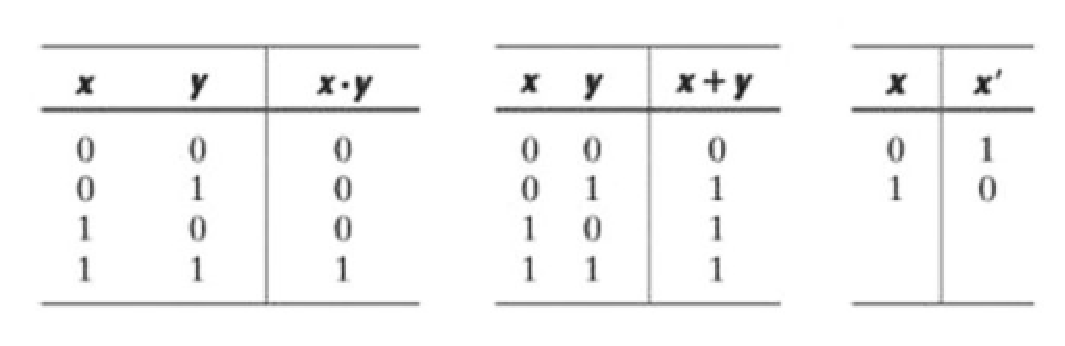
\includegraphics[height=2.0cm]{./images/bao.eps}					\vspace{1pt}
		\end{figure}
	\end{itemize}
	Y demostrando los postulados de Hungtinton, se crea el \'Algebra Booleana de dos valores. Ver p\'agina 42 del libro "Dise\~no Digital".
\end{frame}

\begin{frame}{Teoremas del \'Algebra Booleana}
\frametitle{Teoremas del \'Algebra Booleana}
Dualidad: Toda expresi\'on derivada de los postulados del \'algebra booleana sigue siendo v\'alida si los operadores y elementos de identidad se intercambian.
	\begin{figure}[h]
		\centering
		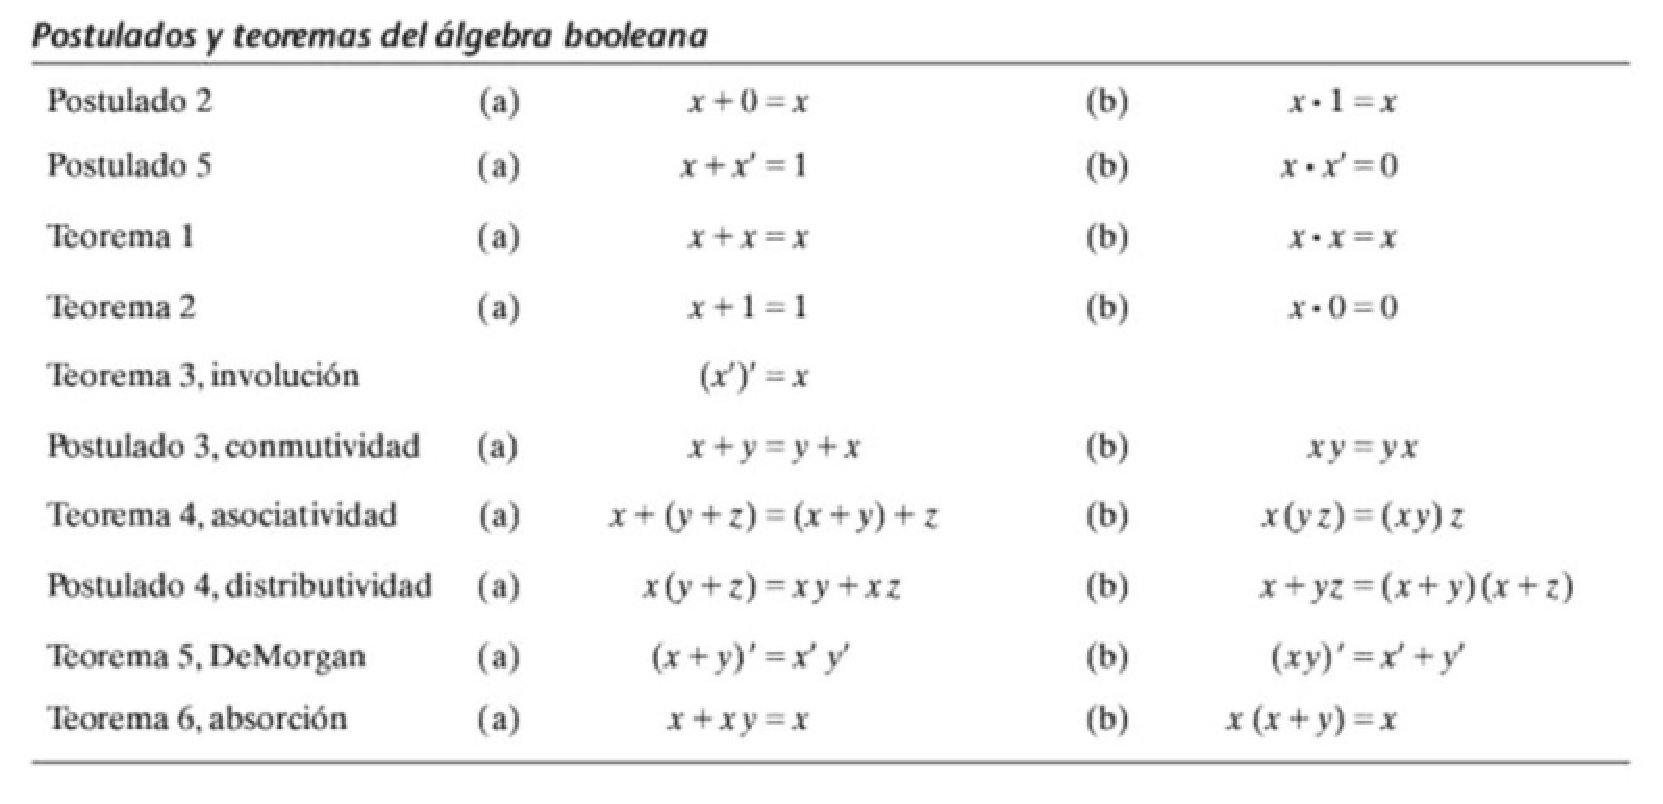
\includegraphics[height=5.0cm]{./images/postulates.eps}
		\vspace{1pt}
	\end{figure}
\end{frame}

\begin{frame}{Precedencia de Operadores}
\frametitle{Precedencia de Operadores}
(1) Par\'entesis.\linebreak
(2) NOT\linebreak
(3) AND\linebreak
(4) OR\linebreak
\end{frame}

\section{Funciones Booleanas}
\begin{frame}{Funciones Booleanas}
\frametitle{Funciones Booleanas}
Analicemos las funciones:
	\begin{itemize}
		\item $F_{1}=x+y'z$
		\item $F_{2}=x'y'z+x'yz+xy'$
	\end{itemize}
\end{frame}

\section{Ejercicios}
\begin{frame}{Ejercicios}
\frametitle{Ejercicios}
Realice los ejercicios 2.2, 2.3, 2.4 y 2.9 del libro "Dise\~no Digital"
\end{frame}

\section{Formas Can\'onicas \& Est\'andar}
\begin{frame}{Formas Can\'onicas \& Est\'andar}
\frametitle{Formas Can\'onicas \& Est\'andar}
Una funci\'on booleana expresada como una suma de  minit\'erminos o producto de maxit\'erminos, est\'a en forma Can\'onica.
	\begin{figure}[h]
		\centering
		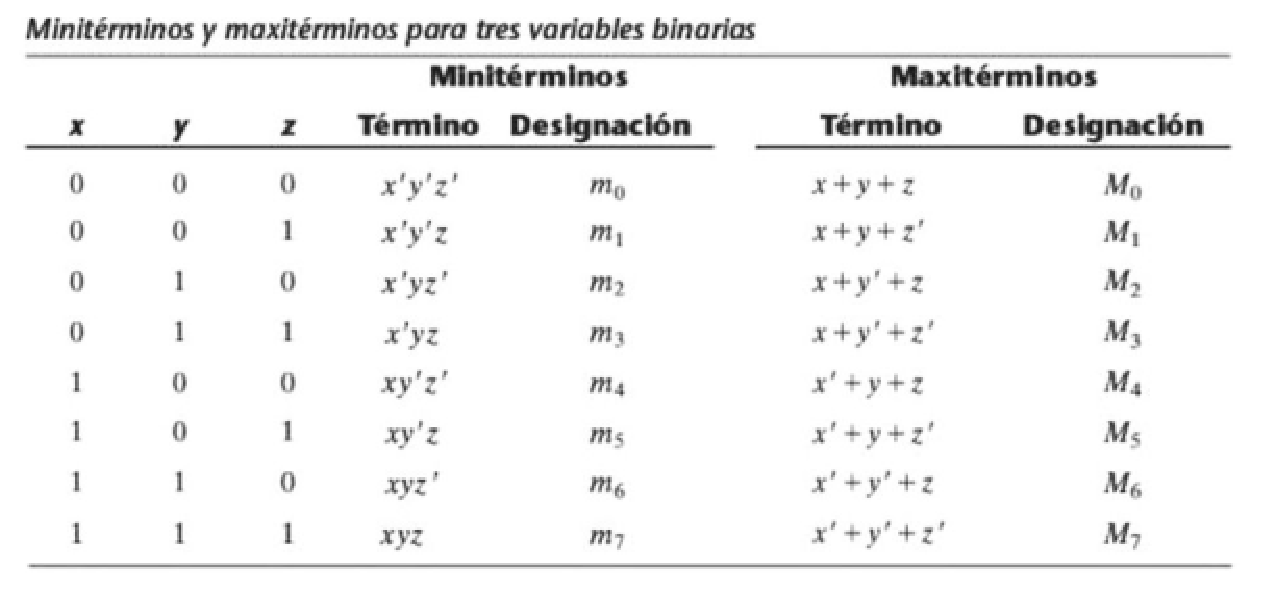
\includegraphics[height=5.0cm]{./images/minmax.eps}
		\vspace{1pt}
	\end{figure}
\end{frame}
\subsection{Desarrollo de ejemplos}
\begin{frame}{Desarrollo de ejemplos}
\frametitle{Desarrollo de ejemplos}
	\begin{enumerate}
		\item Exprese la funci\'on booleana $F=A+B'$ como una suma de mint\'erminos.
		\item Exprese la funci\'on booleana $F=xy+x'z$ como un producto de maxit\'erminos.
	\end{enumerate}
\end{frame}

\section{Familias L\'ogicas Digitales}
\begin{frame}{Familias L\'ogicas Digitales}
\frametitle{Familias L\'ogicas Digitales}
	\begin{enumerate}
		\item TTL: L\'ogica Transistor-Transistor.
		\item ECL: L\'ogica acoplada por emisor.
		\item MOS: Semiconductor de \'oxido de metal.
		\item CMOS: Semiconductor de \'oxido de metal complementario.
	\end{enumerate}
\end{frame}
\begin{frame}{Caracter\'isticas}
\frametitle{Caracter\'isticas}
	\begin{enumerate}
		\item Abanico de entrada o capacidad de entrada.
		\item Disipaci\'on de potencia.
		\item Retardo de propagaci\'on.
		\item Margen de Ruido.
	\end{enumerate}
\end{frame}

\section{Actividades Asincr\'onicas}
\begin{frame}
\frametitle{Actividades Asincr\'onicas}
	\begin{itemize}
		\item Ejercicio o pr\'actica:simplificación de funciones, diagramas l\'ogicos y tablas de verdad.
		\item Juego Did\'actico: \href{https://www.cerebriti.com/juegos-de-tecnologia/algebra-de-boole}{\textcolor{blue}{Link Algebra de Boole}}
	\end{itemize}
\end{frame}

\section{Bibliograf\'ia}
\begin{frame}
	\frametitle{Bibliograf\'ia}
	\begin{itemize}
		\item Morris, M., y Ciletti, M. Diseño Digital, Cap. 2, pág. 38-65.
		\item Argüello D. M, Pérez, S., y Facchini, H. Arquitectura de computadoras, Cap.3, pág. 64-79.
		\end{itemize}
\end{frame}

\end{document}